\begin{figure}[H]
    \centering
    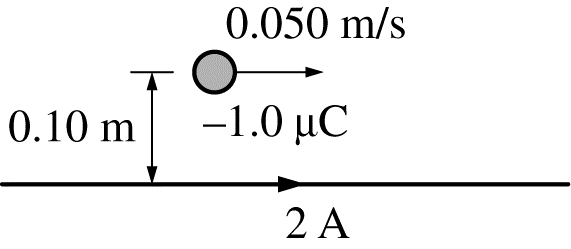
\includegraphics[scale=0.3]{images/img-002-002.png}
\end{figure}

% Multiple Choice Question 1
\begin{questions}\setcounter{question}{0}\question
A small object of charge $-1.0 \unit{\mu C}$ that is $0.10 \unit{m}$ above a long, straight wire moves at a speed of $0.050 \unit{m/s}$ parallel to the wire, as shown in the figure above. The current in the wire is $2 \unit{A}$. What is the magnitude and direction of the magnetic force on the object?

\begin{choices}
\choice $2     \times 10^{-13} \unit{N}$, toward the wire
\choice $2     \times 10^{-13} \unit{N}$, away from the wire
\choice $4 \pi \times 10^{-13} \unit{N}$, toward the wire
\choice $4 \pi \times 10^{-13} \unit{N}$, away from the wire
\choice Zero, direction is undefined
\end{choices}\end{questions}
